\makeatletter
\def\input@path{{../}}
\makeatother
\documentclass[../master_thesis.tex]{subfiles}
\begin{document}
\chapter{Results}\label{chap:Results}
\section{Overview of Tests}
We divided the tests of this implementation into four main types, theoretical
correctness, parametrization, comparison and tests of the variational implementation.

In the tests of theoretical correctness we test if our implementation gives the
results to problems as expected. The tests for this were comparisons to
the energy of  \ce{Li^+} in an environment with dielectric constant $\epsinf = 2$
with the value we would get from the Born model. In the Born model the energy of a  %citation please
one atom ion in a solvent is the same as the energy of a point charge in the same solvent.
This energy is described as
\begin{equation}
  E_{ion} = -\frac{q^{2}}{8 \pi R_{cav}}\left(\frac{1}{\epso\\}-\frac{1}{\epsinf}\right)
\end{equation}
A second comparison with the Born model was done where we tested for the
following relation that should hold for a point charge
\begin{equation}
  \int \gamma_s = \frac{\epsinf - 1}{\epsinf} q
\end{equation}

The parametrization tests were done by changing one parameter at a time while
comparing this same change to Gaussian calculations with different basis sets.
First we only checked the dependency on the radius and how changing it would
affect the reaction field energy with respect to Gaussian calculations of the same
radii. We then compared Gaussian calculations of Radius $R$ against \mrchem
calculations of Radius $R+0.2$ in an attempt to see an improvement in the
results.
A second parametrization test was done with only \ce{Li^+}
where we changed the relative precision of the \mrchem calculations to see how
they affect the energy with respect to the Gaussian energies. This was also done
on different radii.

We then took 4 molecules that were tested by \cite{Chipman2002} and compared the
results from variation of radii against Gaussian results. The molecules used
were \ce{H_2O}, \ce{NO^+}, \ce{CN^-} and \ce{CH_3CONH_2}. These tests are classified into
single cavity tests and \ac{ABC} tests. Single cavity tests are performed in the
same manner as the paramtrization tests where only the radius of the cavity was changed per
calculation. We did not shift the \mrchem calculation's cavity radius.

The \ac{ABC} tests consist of making spherical cavities centered on
each atom with radii equal to their center atom's Van der Waals radius. In this we tested

As stated before in chapters \ref{chap:Solvent_effect} and \ref{chap:implementation}
a variational formulation of the Reaction field Problem was implemented in this thesis,
The tables in Appendix \ref{Datatables} show a row which is labeled "Variational",
though the variational implementation behaved in a irregular way. We will show
the Reaction energy plots for the variational implementation for both water
and \ce{Li^+} as those are the ones that had the most data points. We leave the
reader to evaluate the variational energies for the other molecules.


\section{Data}
The data tables containing all results can be found in appendix \ref{Datatables}, following
tables will show a small sample so the reader can make better understand the tables
in the appendixes.
\subsection{Theoretical correctness Tests}
\subsection{Parametrization Tests}
Wer first variated the Radius of the cavity for water and lithium. The following
table \ref{tab:rawwaterdata}  presents the data for the energy
calculations of \ce{H_2O} with the three first cavity radii as an example of the layout of the
tables.
These are the total  energy of the system including the solvent effect contributions.
The same type of tables were used for the rest of the systems.
\begin{table}[htbp]
  \caption{Total Energy Calculations example for Water in Water. Energy in Hartree and radii of the cavity in Bohr}
  \begin{center}
    \begin{tabular}{|l|r|r|r|r|}
      \hline
      Basis & $R =3.6$ & $R=3.7$ & $R=3.8$ & $\ldots$\\  \hline
      Cc-pVDZ & -7.6039e+01 & -7.6038e+01 & -7.6036e+01 & $\ldots$\\ \hline
      Cc-pVTZ & -7.6070e+01 & -7.6069e+01 & -7.6067e+01 & $\ldots$\\ \hline
      Cc-pVQZ & -7.6078e+01 & -7.6076e+01 & -7.6075e+01 & $\ldots$\\ \hline
      Cc-pV5Z & -7.6080e+01 & -7.6079e+01 & -7.6077e+01 & $\ldots$\\ \hline
      Aug-cc-pVDZ & -7.6054e+01 & -7.6053e+01 & -7.6052e+01 & $\ldots$\\ \hline
      Aug-cc-pVTZ & -7.6074e+01 & -7.6072e+01 & -7.6071e+01 & $\ldots$\\ \hline
      Aug-cc-pVQZ & -7.6079e+01 & -7.6077e+01 & -7.6076e+01 & $\ldots$\\ \hline
      Aug-cc-pV5Z & -7.6080e+01 & -7.6079e+01 & -7.6077e+01 & $\ldots$\\ \hline
      daug-cc-pVDZ & -7.6055e+01 & -7.6053e+01 & -7.6052e+01 & $\ldots$\\ \hline
      daug-cc-pVTZ & -7.6074e+01 & -7.6072e+01 & -7.6071e+01 & $\ldots$\\ \hline
      daug-cc-pVQZ & -7.6079e+01 & -7.6077e+01 & -7.6076e+01 & $\ldots$\\ \hline
      daug-cc-pV5Z & -7.6080e+01 & -7.6079e+01 & -7.6077e+01 & $\ldots$\\ \hline
      mrchem & -7.6085E+01 & -7.6083E+01 & -7.6081E+01 & $\ldots$\\ \hline
    \end{tabular}
  \end{center}
  \label{tab:rawwaterdata}
\end{table}

In order to Calculate the Reaction field energy we took a gas phase calculation
of a basis set and subtracted it from the total energy calculated with the same
basis set. In mrchem this was done using the same relative precision. The
following equation was used to calculate the Reaction field Energy $E_r$
\begin{equation}\label{eq:deltaer}
  E_r = E_{tot} - E_{vac}
\end{equation}
Examples of $E_r$ for the first three cavity radii for water obtained from the operation
in Equation \ref{eq:deltaer} can be seen in table \ref{tab:Erwatdata}

\begin{table}[htbp]
\caption{Reaction Field Energy Calculations example for Water in Water. Energy in Hartree and radii of the cavity in Bohr}
\begin{center}
\begin{tabular}{|l|r|r|r|r|}
\hline
basis & 3.6 & 3.7 & 3.8 & $\ldots$\\ \hline
Cc-pVDZ & -1.2450E-02 & -1.0998E-02 & -9.7804E-03 & $\ldots$\\ \hline
Cc-pVTZ & -1.3097E-02 & -1.1545E-02 & -1.0243E-02 & $\ldots$\\ \hline
Cc-pVQZ & -1.3218E-02 & -1.1651E-02 & -1.0334E-02 & $\ldots$\\ \hline
Cc-pV5Z & -1.3284E-02 & -1.1713E-02 & -1.0393E-02 & $\ldots$\\ \hline
Aug-cc-pVDZ & -1.3190E-02 & -1.1634E-02 & -1.0328E-02 & $\ldots$\\ \hline
Aug-cc-pVTZ & -1.3238E-02 & -1.1670E-02 & -1.0353E-02 & $\ldots$\\ \hline
Aug-cc-pVQZ & -1.3221E-02 & -1.1655E-02 & -1.0338E-02 & $\ldots$\\ \hline
Aug-cc-pV5Z & -1.3223E-02 & -1.1655E-02 & -1.0337E-02 & $\ldots$\\ \hline
daug-cc-pVDZ & -1.3228E-02 & -1.1665E-02 & -1.0351E-02 & $\ldots$\\ \hline
daug-cc-pVTZ & -1.3243E-02 & -1.1675E-02 & -1.0357E-02 & $\ldots$\\ \hline
daug-cc-pVQZ & -1.3223E-02 & -1.1656E-02 & -1.0340E-02 & $\ldots$\\ \hline
daug-cc-pV5Z & -1.3224E-02 & -1.1655E-02 & -1.0337E-02 & $\ldots$\\ \hline
mrchem & -1.8036E-02 & -1.5494E-02 & -1.3437E-02 & $\ldots$\\ \hline
\end{tabular}
\end{center}
\label{tab:Erwatdata}
\end{table}

We now plot the data from the total energy and reaction energy tables for
both water and \ce{Li^+}.

The water plots for the Reaction energy of water for
both the Gaussian and  \mrchem calculations can be seen in Figure \ref{fig:watEnergyplots}.
The same type of plots for \ce{Li^+} can be seen in Figure \ref{fig:lipEnergyplots}.
In both of these figure we are comparing the energy from \mrchem to sets of four
curves formed each of double, triple, quadruple and quintuple zeta Dunning's correlation
consistent \cite{doi:10.1063/1.456153} basis sets as implemented in Gaussian \cite{G09}.
In the first plot we have energies calculated with standard correlation consistent ,
in the second we have augmented, and in the third of each figure we have double augmented.


\begin{figure}[h!]
  \centering
  \begin{subfigure}[b]{0.75\linewidth}
    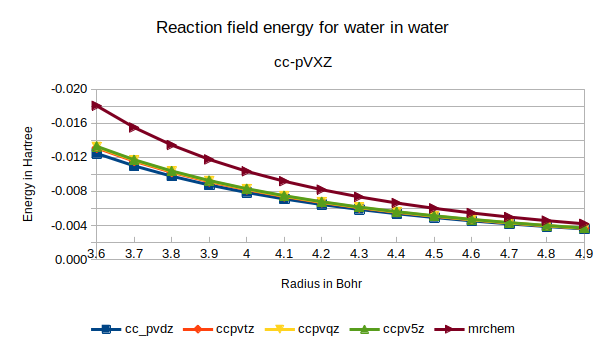
\includegraphics[width=\linewidth]{img/Erwat.png}
  \end{subfigure}
  \begin{subfigure}[b]{0.75\linewidth}
    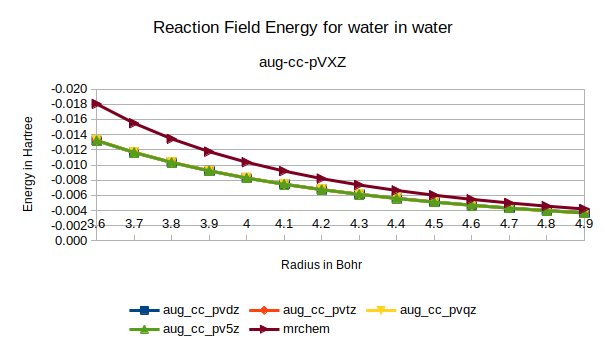
\includegraphics[width=\linewidth]{img/Eraugwat.png}
  \end{subfigure}
  \begin{subfigure}[b]{0.75\linewidth}
    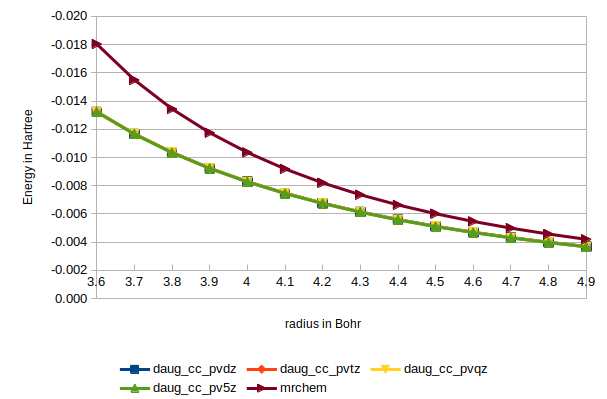
\includegraphics[width=\linewidth]{img/Erdaugwat.png}
  \end{subfigure}
  \caption{Reaction field energy of Water in a water solution, calculated with relative precision $e-05$ in mrchem
  and with different basis sets in Gaussian}
  \label{fig:watEnergyplots}
\end{figure}

\begin{figure}[h!]
  \centering
  \begin{subfigure}[b]{0.75\linewidth}
    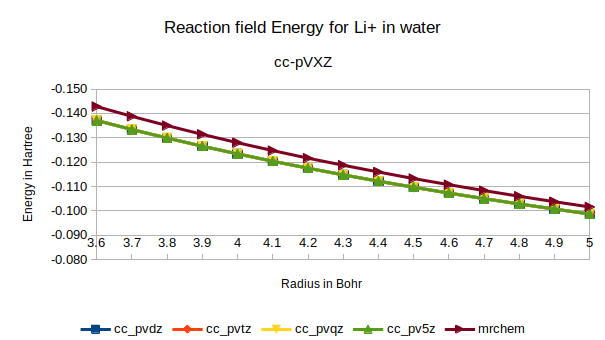
\includegraphics[width=\linewidth]{img/Erlip.png}
  \end{subfigure}
  \begin{subfigure}[b]{0.75\linewidth}
    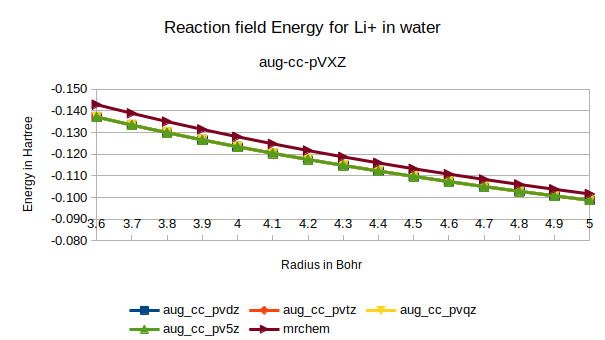
\includegraphics[width=\linewidth]{img/Erauglip.png}
  \end{subfigure}
  \begin{subfigure}[b]{0.75\linewidth}
    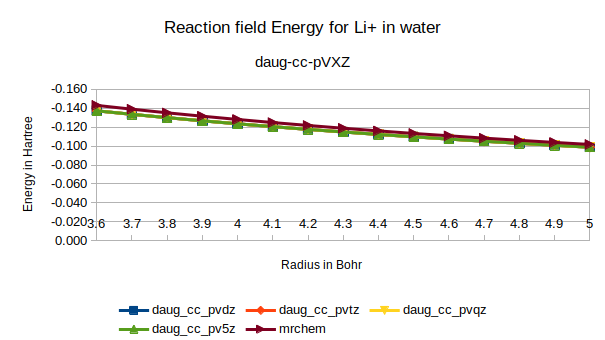
\includegraphics[width=\linewidth]{img/Erdauglip.png}
  \end{subfigure}
  \caption{Reaction field energy of \ce{Li^+} in a water solution, calculated with relative precision $e-05$ in mrchem
  and with different basis sets in Gaussian}
  \label{fig:lipEnergyplots}
\end{figure}

The \mrchem energy values $E_{Mrchem}$ for each radii were compared to the
corresponding values of each of the different basis set calculations in
Gaussian  $E_{Gaussian}^{basis}$ by finding the relative difference $d_r$
between them as
\begin{equation}\label{eq:reldiff}
  d_r = \frac{E_{Gaussian}^{basis} - E_{Mrchem}}{E_{Mrchem}}
\end{equation}
The operation in Equation \ref{eq:reldiff} was applied to all the values for all the
substrate molecules, giving the following figures \ref{fig:watreldiff} and \ref{fig:lipreldiff}.
As before we separated the figures into three plots of four calculations with each
their basis set. First standad correlation consistent, then augmented and lastly double augmented
with double, triple, quadruple and quintuple zeta calculation for each of the plots.

\begin{figure}[h!]
  \centering
  \begin{subfigure}[b]{0.75\linewidth}
    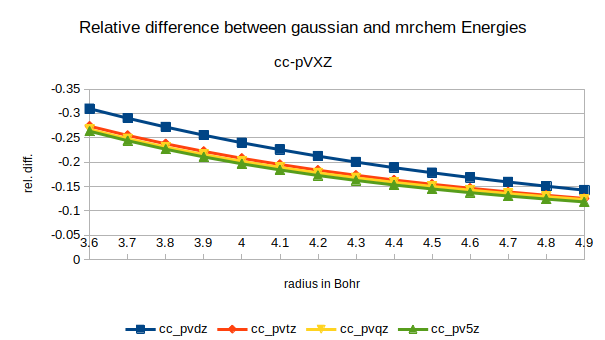
\includegraphics[width=\linewidth]{img/watreldiff.png}
  \end{subfigure}
  \begin{subfigure}[b]{0.75\linewidth}
    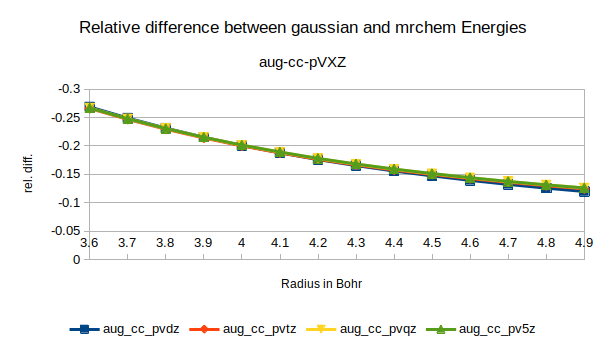
\includegraphics[width=\linewidth]{img/wataugreldiff.png}
  \end{subfigure}
  \begin{subfigure}[b]{0.75\linewidth}
    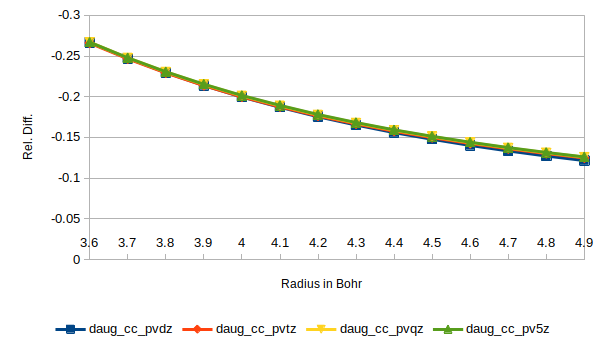
\includegraphics[width=\linewidth]{img/watdaugreldiff.png}
  \end{subfigure}
  \caption{Relative difference between the Reaction field energy of Water in a water solution calculated with with relative precision $e-05$ in \mrchem
   and with different basis sets in Gaussian}
  \label{fig:watreldiff}
\end{figure}



We then shifted the cavity radius of the mrchem calculations for both water and
\ce{Li^+} so they were $0.2$ Bohr bigger and compared them to Gaussian calculations
with an unshifted Radius. The relative Difference plots for water and \ce{Li^+} can be seen
in Figures \ref{fig:watreldiff02} and \ref{fig:lipreldiff02} respectivelly.

\begin{figure}[h!]
  \centering
  \begin{subfigure}[b]{0.75\linewidth}
    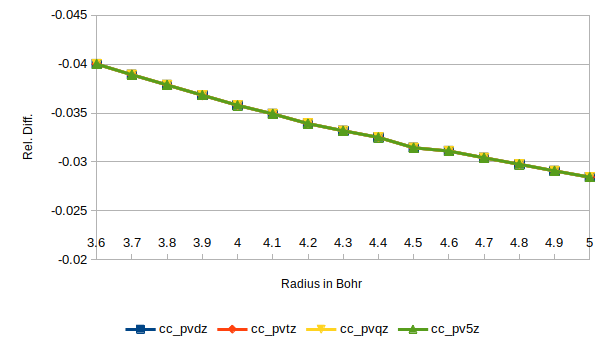
\includegraphics[width=\linewidth]{img/lipreldiff.png}
  \end{subfigure}
  \begin{subfigure}[b]{0.75\linewidth}
    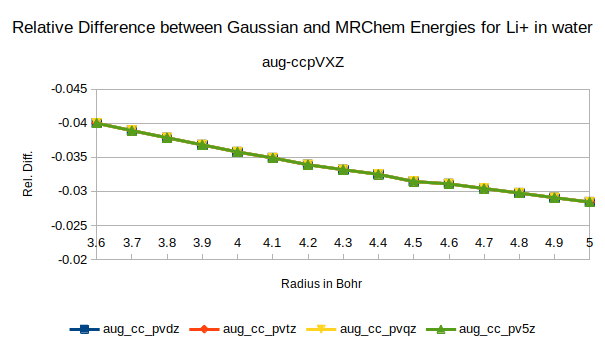
\includegraphics[width=\linewidth]{img/lipaugreldiff.png}
  \end{subfigure}
  \begin{subfigure}[b]{0.75\linewidth}
    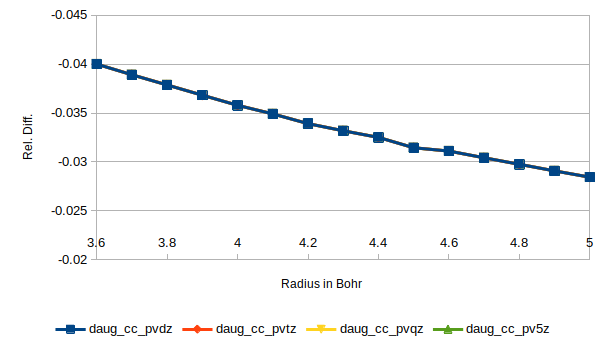
\includegraphics[width=\linewidth]{img/lipdaugreldiff.png}
  \end{subfigure}
  \caption{Relative difference between the Reaction field energy of\ce{Li^+} in a water solution calculated with relative precision $e-05$ in \mrchem
  and with different basis sets in Gaussian}
  \label{fig:lipreldiff}
\end{figure}

\begin{figure}[h!]
  \centering
  \begin{subfigure}[b]{0.75\linewidth}
    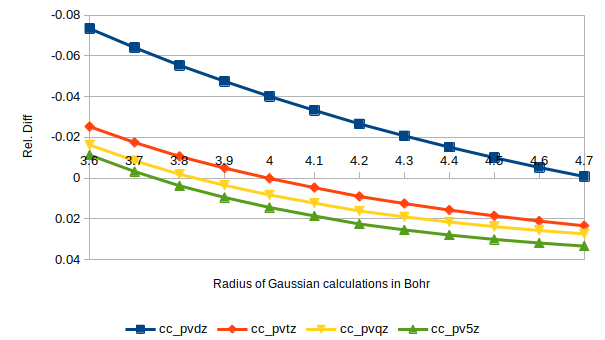
\includegraphics[width=\linewidth]{img/watreldiff02.png}
  \end{subfigure}
  \begin{subfigure}[b]{0.75\linewidth}
    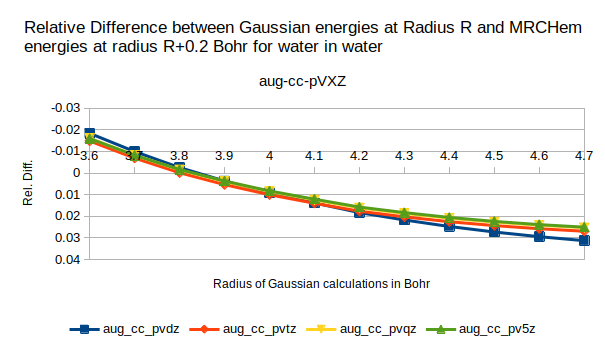
\includegraphics[width=\linewidth]{img/wataugreldiff02.png}
  \end{subfigure}
  \begin{subfigure}[b]{0.75\linewidth}
    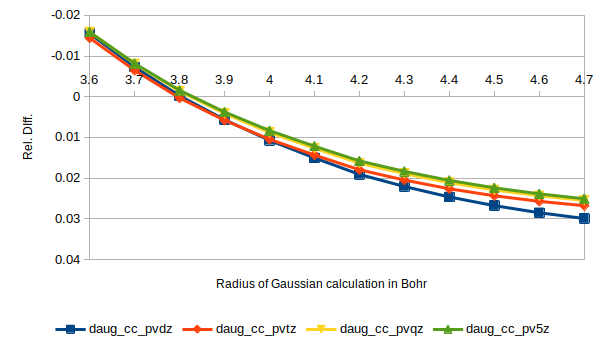
\includegraphics[width=\linewidth]{img/watdaugreldiff02.png}
  \end{subfigure}
  \caption{Relative difference between the Reaction field energy of Water in a water solution calculated with with relative precision $e-05$ in \mrchem
  and with different basis sets in Gaussian}
  \label{fig:watreldiff02}
\end{figure}

\begin{figure}[h!]
  \centering
  \begin{subfigure}[b]{0.75\linewidth}
    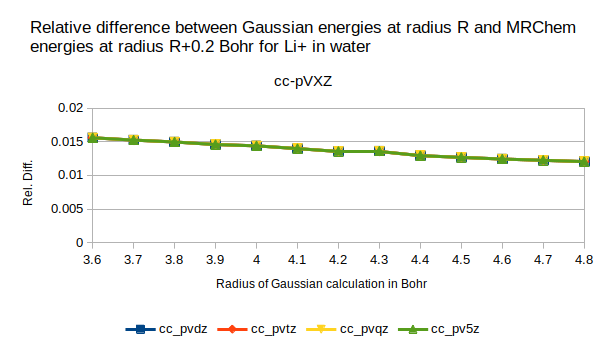
\includegraphics[width=\linewidth]{img/lipreldiff02.png}
  \end{subfigure}
  \begin{subfigure}[b]{0.75\linewidth}
    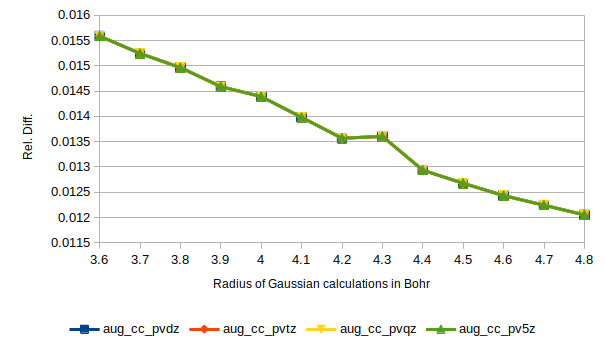
\includegraphics[width=\linewidth]{img/lipaugreldiff02.png}
  \end{subfigure}
  \begin{subfigure}[b]{0.75\linewidth}
    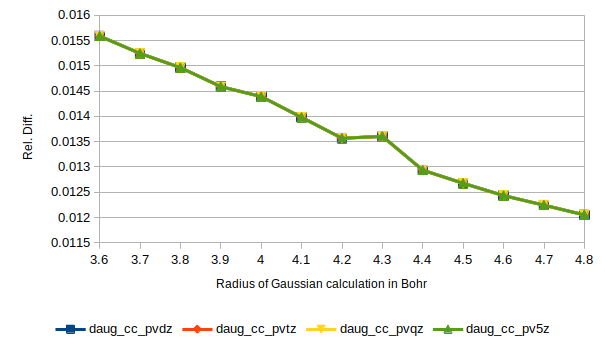
\includegraphics[width=\linewidth]{img/lipdaugreldiff02.png}
  \end{subfigure}
  \caption{Relative difference between the Reaction field energy of \ce{Li^+} in a water solution calculated with relative precision $e-05$ in \mrchem
  and with different basis sets in Gaussian}
  \label{fig:lipreldiff02}
\end{figure}

Lastly we computed the reaction field energies of \ce{Li^+} with four different
relative precisions; $1e-3, 1e-4, 1e-5,\  \text{and}\  1e-6$. We compared these
to the reaction field energies calculated with the most complete basis set:
\verb!daug-cc-pV5Z! as described in
\begin{equation}\label{eq:difgauss}
    d_r = \frac{E_{Li^+} - E_{Gaussian}}{E_{Gaussian}}
\end{equation}
Figure \ref{fig:lipprecreldef} shows the plots of the operation in Equation \ref{eq:difgauss} above.
First all of the relative differences plotted together, then the second one contains
only the results for relative precision $1e(-4), 1e(-5),\  \text{and}\  1e(-6)$ since
the results with relative precission $1e(-3)$ are over five times larger than the other ones.

\begin{figure}[h!]
  \centering
  \begin{subfigure}[b]{0.75\linewidth}
    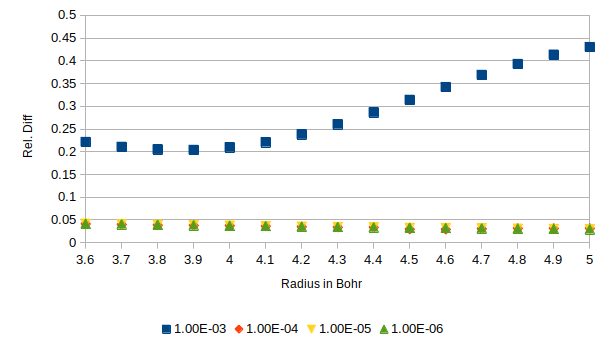
\includegraphics[width=\linewidth]{img/lipprecallreldiff.png}
  \end{subfigure}
  \begin{subfigure}[b]{0.75\linewidth}
    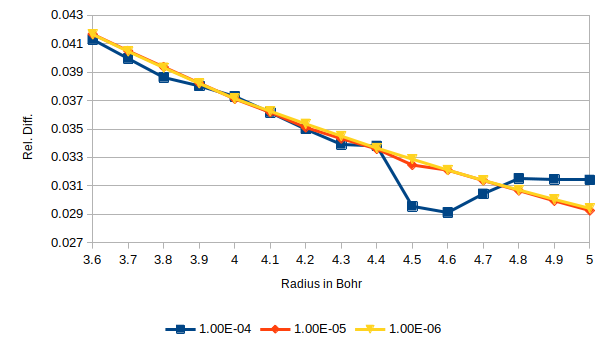
\includegraphics[width=\linewidth]{img/lipprecallreldiffexcl.png}
  \end{subfigure}
  \caption{Relative difference between the Reaction field energy of \ce{Li^+} in a water solution calculated with different relative precisions in \mrchem  and same calculations in Gaussian with daug-cc-pV5Z}
  \label{fig:lipprecreldef}
\end{figure}

\subsection{Comparison Tests}

These tests were divided into single cavity and \ac{ABC} tets. The single cavity
tests are the same type of tests performed on water in the prvoius sections. These
were tests were applied to \ce{NO^+}  and \ce{CN^-}. We did not apply this test
on \ce{CH_3CONH_2} as the size of the melcule made the calculations in both Gaussian
and \mrchem extremely slow.

Following are figures \ref{fig:nopEnergyplots} and \ref{fig:cyanEnergyplots}
that show the energies of the mrchem calculations plotted
against the energies from the Gaussian calculation for water, \ce{NO^+}, and
\ce{CN^-} respectively. Many of the Mrchem results for \ce{CN^-} and \ce{NO^+}
around the interval $(4.0, 4.5)$ diverged and finished or never finished
running due to divergence,  these results were therefore removed from the figures so as to facilitate
the visualization of the trends across the radii. The values which deverged but still
finished running can be viewed in section \ref{Datatables}.



\begin{figure}[h!]
  \centering
  \begin{subfigure}[b]{0.75\linewidth}
    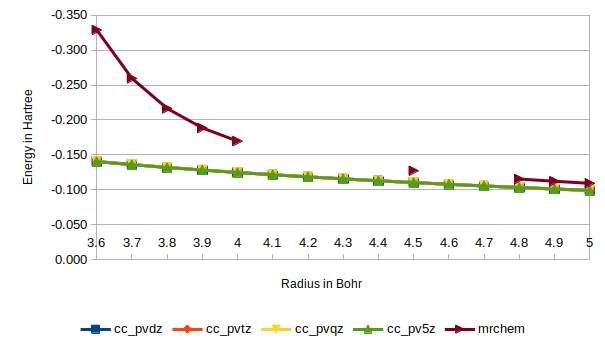
\includegraphics[width=\linewidth]{img/Ernop.png}
  \end{subfigure}
  \begin{subfigure}[b]{0.75\linewidth}
    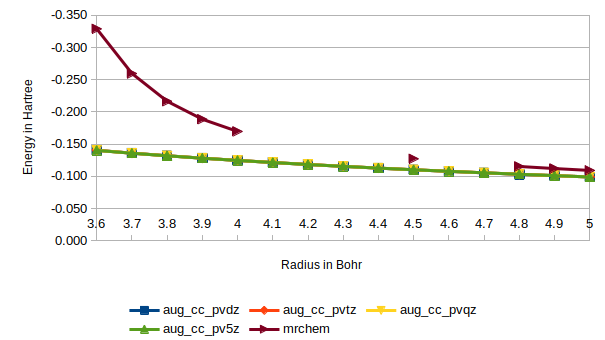
\includegraphics[width=\linewidth]{img/Eraugnop.png}
  \end{subfigure}
  \begin{subfigure}[b]{0.75\linewidth}
    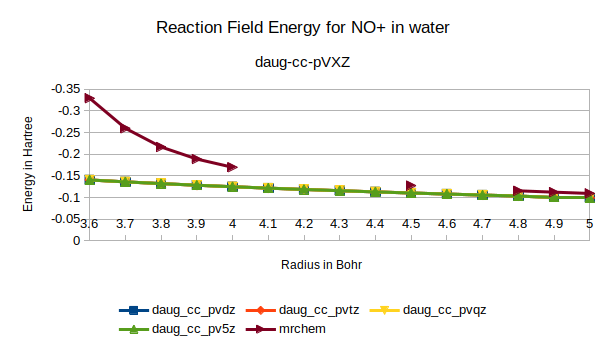
\includegraphics[width=\linewidth]{img/Erdaugnop.png}
  \end{subfigure}
  \caption[Energy plots for \ce{NO^+}]{Reaction field energy of \ce{NO^+} in a water solution, calculated with mrchem
  and with different basis sets in Gaussian}
  \label{fig:nopEnergyplots}

\end{figure}
\begin{figure}[h!]
  \centering
  \begin{subfigure}[b]{0.75\linewidth}
    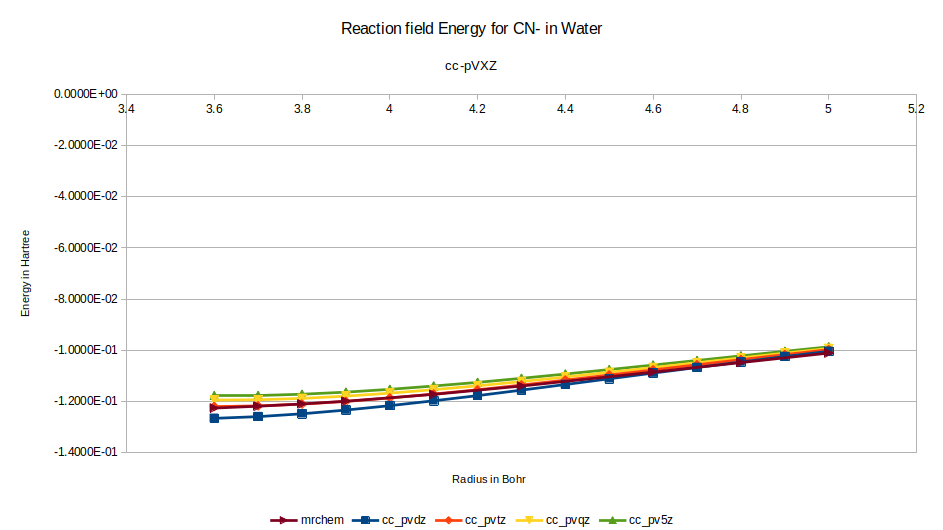
\includegraphics[width=\linewidth]{img/Ercyan.png}
  \end{subfigure}
  \begin{subfigure}[b]{0.75\linewidth}
    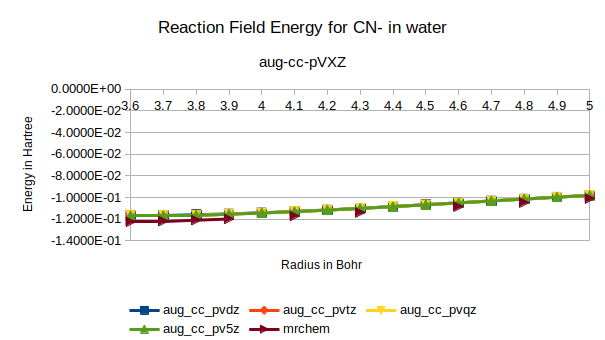
\includegraphics[width=\linewidth]{img/Eraugcyan.png}
  \end{subfigure}
  \begin{subfigure}[b]{0.75\linewidth}
    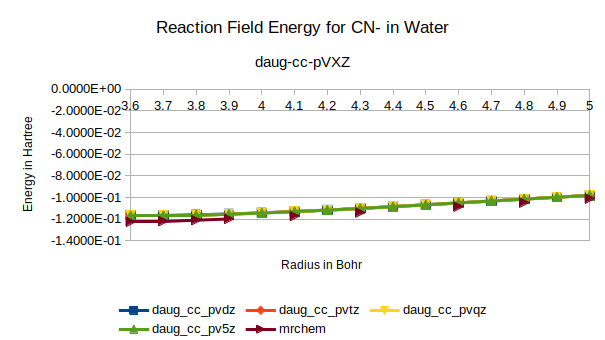
\includegraphics[width=\linewidth]{img/Erdaugcyan.png}
  \end{subfigure}
  \caption{Reaction field energy of \ce{CN^-} in a water solution, calculated with mrchem
  and with different basis sets in Gaussian}
  \label{fig:cyanEnergyplots}
\end{figure}

The Figures \ref{fig:nopreldiff} and \ref{fig:cyanreldiff} show the relative
difference between the Gaussian and \mrchem results as shown in Equation \ref{eq:reldiff}


\begin{figure}[h!]
  \centering
  \begin{subfigure}[b]{0.75\linewidth}
    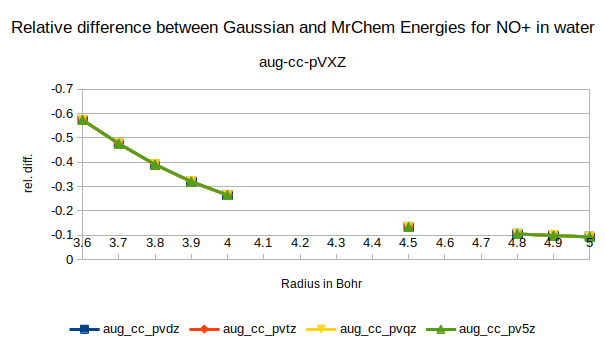
\includegraphics[width=\linewidth]{img/nopreldiff.png}
  \end{subfigure}
  \begin{subfigure}[b]{0.75\linewidth}
    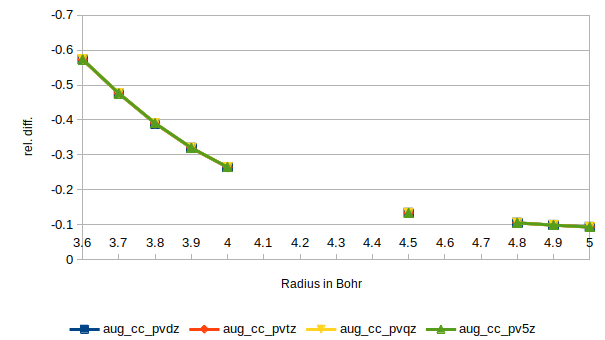
\includegraphics[width=\linewidth]{img/nopaugreldiff.png}
  \end{subfigure}
  \begin{subfigure}[b]{0.75\linewidth}
    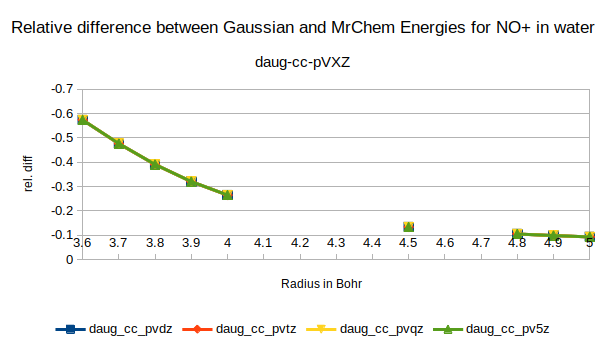
\includegraphics[width=\linewidth]{img/nopdaugreldiff.png}
  \end{subfigure}
  \caption{Relative difference between the Reaction field energy of \ce{NO^+} in a water solution calculated with MrChem
  and with different basis sets in Gaussian}
  \label{fig:nopreldiff}
\end{figure}

\begin{figure}[h!]
  \centering
  \begin{subfigure}[b]{0.75\linewidth}
    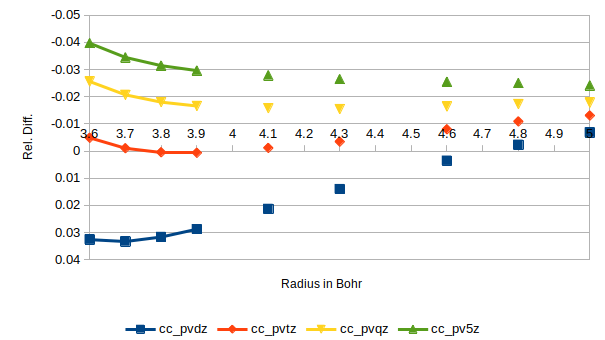
\includegraphics[width=\linewidth]{img/cyanreldiff.png}
  \end{subfigure}
  \begin{subfigure}[b]{0.75\linewidth}
    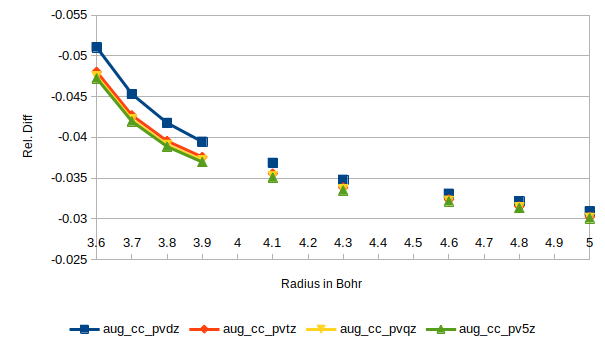
\includegraphics[width=\linewidth]{img/cyanaugreldiff.png}
  \end{subfigure}
  \begin{subfigure}[b]{0.75\linewidth}
    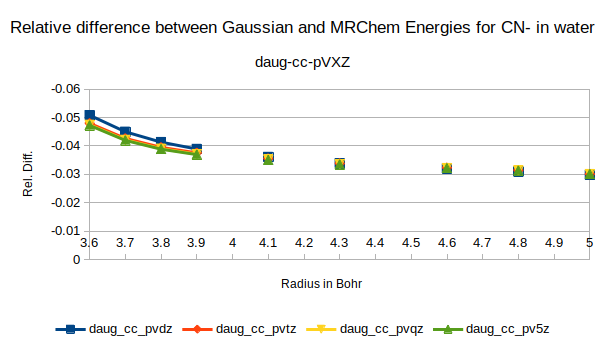
\includegraphics[width=\linewidth]{img/cyandaugreldiff.png}
  \end{subfigure}
  \caption{Relative difference between the Reaction field energy of \ce{CN^-} in a water solution calculated with MrChem
  and with different basis sets in Gaussian}
  \label{fig:cyanreldiff}
\end{figure}

Since the \ac{ABC} tests were just two data points for each basis set and \newline\mrchem
we will present them in a tabulated manner. Here we did tests for \ce{CH_3CONH_2}, \ce{H_2O}, \ce{CN^-} and \ce{NO^+}
for both the Bondi Van der Waals radii and the same radii shifted by $0.2$ Bohr as was done preiously.

Tables \ref{tab:watabcreldiff}, \ref{tab:nopabcreldiff}, \ref{tab:cyanabcreldiff}, \ref{tab:acetamidabcreldiff}
each show the relative difference for the \ac{ABC} and shifted \ac{ABC} tests
for \ce{H_20}, \ce{NO^+}, \ce{CN^-}, and \ce{CH_3CONH_2} respectivelly. The
total and  reaction field energy for each of these can be seen in appendix \ref{Datatables}.

The shifted \ac{ABC} did not converge for \ce{CN^-}, so a comparison between the two sets
of radii is not possible, we can still compare with the basis sets and see how it compared with
the rest of the single cavity values.

The \verb!daug-cc-pV5Z! Gaussian calculations for \ce{CH_3CONH_2} did not finish
after $72$ hours of running. We will therefore present the comparison to the other
basis sets and not include this one.

\begin{table}[htbp]
\caption{Relative difference between Gaussian and \mrchem results from \ac{ABC}  test for water}
\begin{tabular}{|l|r|r|}
\hline
basis & \multicolumn{1}{l|}{Van der Waals} & \multicolumn{1}{l|}{Van der Waals + 0.2 Bohr} \\ \hline
Cc-pVDZ & -0.150906543613475 & -0.141285964520019 \\ \hline
Cc-pVTZ & -0.128295351717095 & -0.119975293105413 \\ \hline
Cc-pVQZ & -0.12895264591432 & -0.120205694685673 \\ \hline
Cc-pV5Z & -0.129254059406516 & -0.119768698510995 \\ \hline
Aug-cc-pVDZ & -0.12913031667549 & -0.119600162056159 \\ \hline
Aug-cc-pVTZ & -0.134287756186553 & -0.124924550255723 \\ \hline
Aug-cc-pVQZ & -0.136838481699817 & -0.127632128628228 \\ \hline
Aug-cc-pV5Z & -0.136314953280294 & -0.12750818602861 \\ \hline
daug-cc-pVDZ & -0.128163492341195 & -0.119393048377284 \\ \hline
daug-cc-pVTZ & -0.133787441562788 & -0.124631587509391 \\ \hline
daug-cc-pVQZ & -0.136489745183213 & -0.127307230549555 \\ \hline
daug-cc-pV5Z & -0.136235086647362 & -0.127443949643962 \\ \hline
\end{tabular}
\label{tab:watabcreldiff}
\end{table}

\begin{table}[htbp]
\caption{Relative difference between Gaussian and \mrchem results from \ac{ABC}  test for \ce{NO^+}}
\begin{tabular}{|l|r|r|}
\hline
basis & \multicolumn{1}{l|}{Van der Waals} & \multicolumn{1}{l|}{Van der Waals + 0.2 Bohr} \\ \hline
Cc-pVDZ & -3.5984E-02 & -3.4028E-02 \\ \hline
Cc-pVTZ & -3.6922E-02 & -3.4965E-02 \\ \hline
Cc-pVQZ & -3.7470E-02 & -3.5239E-02 \\ \hline
Cc-pV5Z & -3.8105E-02 & -3.5695E-02 \\ \hline
Aug-cc-pVDZ & -3.9069E-02 & -3.6582E-02 \\ \hline
Aug-cc-pVTZ & -3.8020E-02 & -3.5793E-02 \\ \hline
Aug-cc-pVQZ & -3.7927E-02 & -3.5622E-02 \\ \hline
Aug-cc-pV5Z & -3.8146E-02 & -3.5744E-02 \\ \hline
daug-cc-pVDZ & -3.8974E-02 & -3.6432E-02 \\ \hline
daug-cc-pVTZ & -3.8111E-02 & -3.5798E-02 \\ \hline
daug-cc-pVQZ & -3.7998E-02 & -3.5663E-02 \\ \hline
daug-cc-pV5Z & -3.8139E-02 & -3.5740E-02 \\ \hline
\end{tabular}
\label{tab:nopabcreldiff}
\end{table}

\begin{table}[htbp]
\caption{Relative difference between Gaussian and \mrchem results from \ac{ABC}  test for \ce{CN^-}}
\begin{tabular}{|l|r|}
\hline
basis & \multicolumn{1}{l|}{Van der Waals} \\ \hline
Cc-pVDZ & 0.01805797 \\ \hline
Cc-pVTZ & 0.00402722 \\ \hline
Cc-pVQZ & -0.00689520 \\ \hline
Cc-pV5Z & -0.01760704 \\ \hline
Aug-cc-pVDZ & -0.02534307 \\ \hline
Aug-cc-pVTZ & -0.02484616 \\ \hline
Aug-cc-pVQZ & -0.02473155 \\ \hline
Aug-cc-pV5Z & -0.02453156 \\ \hline
daug-cc-pVDZ & -0.02428967 \\ \hline
daug-cc-pVTZ & -0.02475331 \\ \hline
daug-cc-pVQZ & -0.02472359 \\ \hline
daug-cc-pV5Z & -0.02449823 \\ \hline
\end{tabular}
\label{tab:cyanabcreldiff}
\end{table}

\begin{table}[htbp]
\caption{Relative difference between Gaussian and \mrchem results from \ac{ABC}  test for \ce{CH_3CONH_2}}
\begin{tabular}{|l|r|r|}
\hline
basis & \multicolumn{1}{l|}{vdw} & \multicolumn{1}{l|}{Vdw+0.2} \\ \hline
Cc-pVDZ & -0.186177328600554 & -0.179892322986873 \\ \hline
Cc-pVTZ & -0.13954657945224 & -0.131024507798636 \\ \hline
Cc-pVQZ & -0.12431319516031 & -0.113411992173209 \\ \hline
Cc-pV5Z & -0.12131273376434 & -0.109744750765678 \\ \hline
Aug-cc-pVDZ & -0.113966441504817 & -0.103344765190205 \\ \hline
Aug-cc-pVTZ & -0.120388767462925 & -0.108539852800393 \\ \hline
Aug-cc-pVQZ & -0.122585402181545 & -0.110802064126041 \\ \hline
Aug-cc-pV5Z & -0.122435027608944 & -0.110977017225698 \\ \hline
daug-cc-pVDZ & -0.117198265984418 & -0.107083369948664 \\ \hline
daug-cc-pVTZ & -0.121288328616877 & -0.109694324315186 \\ \hline
daug-cc-pVQZ & -0.122478065257119 & -0.110807811509374 \\ \hline
\end{tabular}
\label{tab:acetamidabcreldiff}
\end{table}



\subsection{Variational implementation Tests}
Figures \ref{fig:watvarEr} and \ref{fig:lipvarEr} show the reaction field energy
calculated with the variational implementation for water and \ce{Li^+}
respectivelly. Figures \ref{fig:watreldiff} and \ref{fig:lipreldiff} show the
relative difference as calculated with Equation \ref{eq:reldiff} for water and \ce{Li^+}
respectivelly.

\begin{figure}[h!]
  \centering
  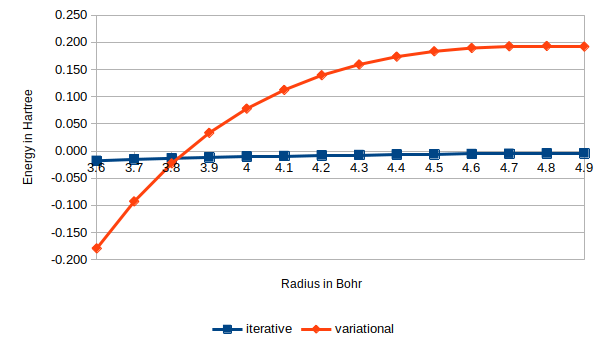
\includegraphics[width=0.75\linewidth]{img/watvarEr.png}
  \caption{Relative difference between the Reaction field energy of \ce{CN^-} in a water solution calculated with MrChem
  and with different basis sets in Gaussian}
  \label{fig:watvarEr}
\end{figure}

\begin{figure}[h!]
  \centering
  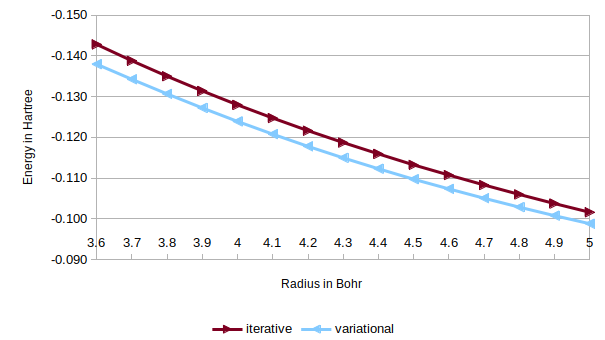
\includegraphics[width=0.75\linewidth]{img/lipvarEr.png}
  \caption{Relative difference between the Reaction field energy of \ce{CN^-} in a water solution calculated with MrChem
  and with different basis sets in Gaussian}
  \label{fig:lipvarEr}
\end{figure}

\begin{figure}[h!]
  \centering
  \begin{subfigure}[b]{0.75\linewidth}
    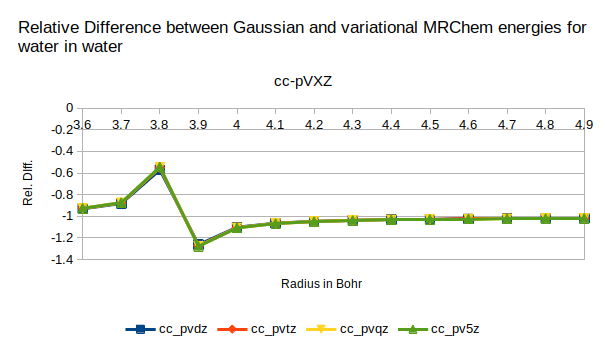
\includegraphics[width=\linewidth]{img/watvarreldiff.png}
  \end{subfigure}
  \begin{subfigure}[b]{0.75\linewidth}
    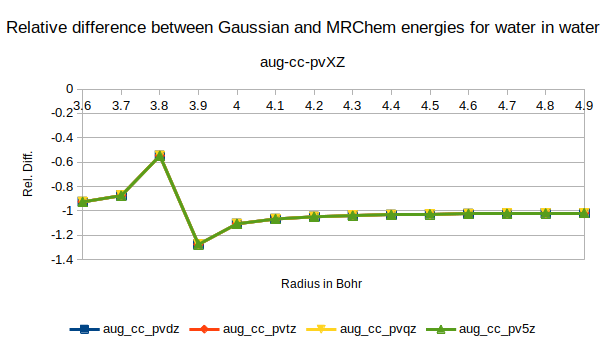
\includegraphics[width=\linewidth]{img/watvaraugreldiff.png}
  \end{subfigure}
  \begin{subfigure}[b]{0.75\linewidth}
    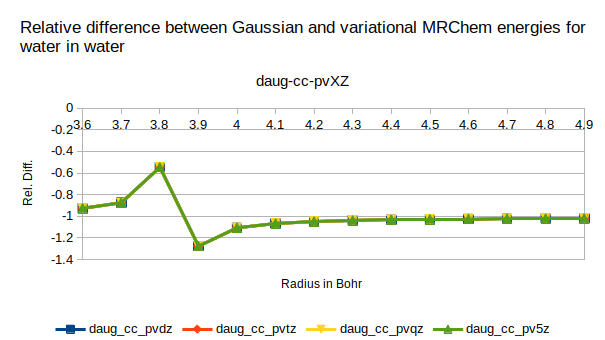
\includegraphics[width=\linewidth]{img/watvardaugreldiff.png}
  \end{subfigure}
  \caption{Relative difference between the Reaction field energy of \ce{CN^-} in a water solution calculated with MrChem
  and with different basis sets in Gaussian}
  \label{fig:watreldiff}
\end{figure}

\begin{figure}[h!]
  \centering
  \begin{subfigure}[b]{0.75\linewidth}
    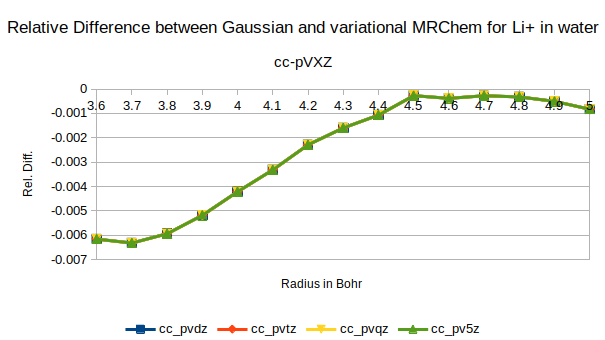
\includegraphics[width=\linewidth]{img/lipvarreldiff.png}
  \end{subfigure}
  \begin{subfigure}[b]{0.75\linewidth}
    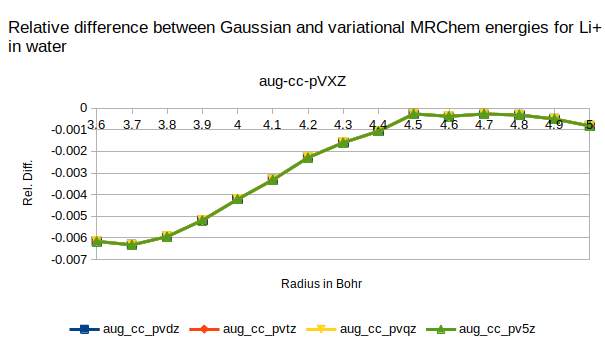
\includegraphics[width=\linewidth]{img/lipvaraugreldiff.png}
  \end{subfigure}
  \begin{subfigure}[b]{0.75\linewidth}
    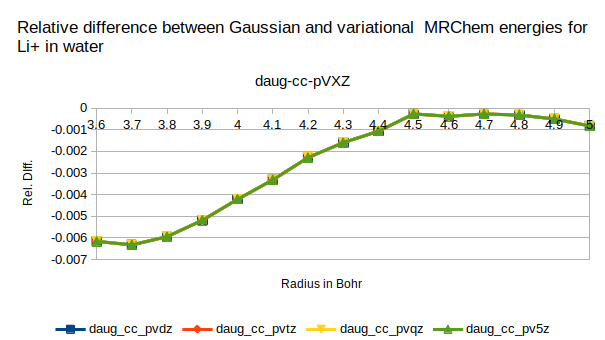
\includegraphics[width=\linewidth]{img/lipvardaugreldiff.png}
  \end{subfigure}
  \caption{Relative difference between the Reaction field energy of \ce{CN^-} in a water solution calculated with MrChem
  and with different basis sets in Gaussian}
  \label{fig:lipreldiff}
\end{figure}

\section{Discussion}
\section{Conclusion}
\section{Areas of improvement/future development}




\begin{acronym}
\acro{AUS}[\href{https://www.sigma2.no/content/advanced-user-support}{AUS}]{Numerical Methods in Quantum Chemistry}
\acro{BO}{Born-Oppenheimer}
\acro{CTCC}[\href{http://www.ctcc.no}{CTCC}]{Centre for Theoretical and Computational Chemistry}
\acro{DC}{Dielectric Continuum}
\acro{DFT}{Density Functional Theory}
\acro{EFP}{Effective Fragment Potential}
\acro{EU}{European Union}
\acro{HF}{Hartree-Fock}
\acro{Hylleraas}[\href{https://www.mn.uio.no/hylleraas/english/}{Hylleraas}]{Hylleraas
  Centre for Quantum Molecular Sciences}
\acro{HPC}{High Performance Computing}
\acro{KTH}{Royal Institute of Technology}
\acro{LDA}{Local Density Approximation}
\acro{MCD}{Magnetic Circular Dichroism}
\acro{MCSCF}{Multiconfiguration Self Consistent Field}
\acro{MM}{Molecular Mechanics}
\acro{MW}{Multiwavelet}
\acro{NFR}{Norwegian Research Council}
\acro{NMQC}[\href{http://www.ctcc.no/events/conferences/2015/numeric-conference/}{NMQC}]{Numerical Methods in Quantum Chemistry}
\acro{NOTUR}[\href{https://www.notur.no/}{NOTUR}]{Norwegian Metacenter for Computational Science}
\acro{PCM}{Polarizable Continuum Model}
\acro{PI}{Primcipal Investigator}
\acro{QC}{Quantum Chemistry}
\acro{QM}{Quantum Mechanics}
\acro{QM/MM}{Quantum Mechanics/Molecular Mechanics}
\acro{ROA}{Raman Optical Activity}
\acro{SC}{semiconductor}
\acro{SCF}{Self Consistent Field}
\acro{SHG}{Second Harmonic Genertation}
\acro{STSM}{Short-term scientific mission}
\acro{TPA}{Two-Photon Absorption}
\acro{WP}{Work Package}
\acro{CBS}{Complete Basis Set}
\acro{TCG}{Theoretical Chemistry Group}
\acro{vdW}{van der Waals}
\acro{SE}{Schrödinger Equation}
\acro{PES}{Potential Energy Surface}
\acro{LCAO}{Linear Combination of Atomic Orbitals}
\acro{MRA}{Multi-Resolution Analysis}
\acro{NS}{Nonstandard}
\end{acronym}

\biblio
\end{document}
